\documentclass[11pt]{article}
\usepackage[a4paper,margin=23mm]{geometry}
\usepackage[T1]{fontenc}
\usepackage[section]{placeins}
\usepackage{lmodern,graphicx,booktabs,longtable,amsmath,amssymb,xcolor,hyperref,float}
\hypersetup{colorlinks=true,linkcolor=blue,urlcolor=blue,citecolor=blue}
\setlength{\parindent}{0pt}\setlength{\parskip}{5pt}
\title{Optimizer Sensitivity and Candidate Selection in Noise-Aware Quantum Circuit Search}
\author{Anonymous manuscript}
\date{Revision 3.0.0 --- 21 October 2026}
\begin{document}\maketitle
\begin{abstract}We examine how optimizer choice and candidate selection affect a corrected noise-aware quantum architecture-search implementation. Development seeds select optimizer and generic search-control settings; a frozen protocol then evaluates seven methods on three fixed synthetic GHZ tasks with 32 fresh paired seeds and 100 noise scenarios per regime. The study contains 672 main runs, 64 secondary ablation runs, and 108 development runs. Only the frozen-policy contrast favors D-NCQAS after Holm correction (difference +0.0322; adjusted p=0.0471); the other three primary contrasts are not significant. D-NCQAS has mean task-averaged tail fidelity 0.5049, compared with 0.7865 for a validation-selected analytic tree. A separate molecular optimization study evaluates 120 fixed-ansatz fits using matched starts and cap/refinement controls. All selected BFGS fits meet an independently checked gradient threshold, while 112/120 report solver success. We release configurations, raw observations, checkpoints, diagnostics and executable analyses. The results concern this implementation and budget; they do not establish hardware performance or state-of-the-art superiority.\end{abstract}

\section{Introduction and related work}
Quantum architecture search can use reinforcement learning to construct circuits for state preparation \cite{qas}. Adversarial architect-saboteur training provides a framework for searching under amplified noise \cite{coev}. The present project is a modified reconstruction of that idea, not the official source implementation and not a reproduction of its full benchmark. A prior code audit corrected gradient signs, rollout probabilities, stress projection, topology handling and evaluation pairing. This revision asks whether a numerically correct implementation actually learns, whether its selected circuits outperform meaningful controls, and whether molecular optimizer termination supports the reported energy conclusions.

These questions have substantial precedent. BenchRL-QAS compares multiple reinforcement-learning agents across quantum tasks and highlights task-dependent rankings \cite{bench}. Bi et al. analyze failures of fidelity-driven circuit search and propose entanglement-aware rewards \cite{trap}. We therefore do not claim to discover fidelity traps or to introduce quantum architecture search. Our narrower contribution is a controlled, traceable diagnosis that separates policy movement, typical policy quality, candidate-selection quality and molecular stationarity in one corrected artifact. The generic baselines used here do not replace a full comparison against those authors' implementations.

\section{Scientific model and corrected implementation}
The main tasks are GHZ preparation on a three-qubit chain-shaped tree, a five-qubit branched tree, and a five-qubit chain. Graphs and error rates are synthetic. Exact density matrices model serial gates, local error channels and gate-time phase damping. State fidelity is evaluated before readout; assignment-noisy computational-basis success is a separate observable. Noise scenarios combine heterogeneous rates, discrete Ornstein-Uhlenbeck evolution and stochastic jumps. Nominal, static-stress and OU-stress banks use separate random streams and are generated independently of circuit length. Every method receives the same test-bank configurations for a given task and seed. Each noise evaluation uses the final snapshot of a six-epoch calibration trajectory and holds that configuration fixed during circuit execution; this does not model within-circuit drift or online calibration tracking.

The legal alphabet contains H, X, Z and S on each qubit, CNOT in both directions on every graph edge, fixed RY(pi/2), RZ(pi/4), RX(pi/2), and termination. The maximum length is 2n+2; termination is allowed after n gates. A common mask excludes adjacent self-inverse Clifford pairs. It does not remove every identity-equivalent sequence. The policy observes local Pauli expectations, neighboring ZZ correlations, GHZ populations/coherence and normalized time. These features are not a complete density-matrix representation. A 64-by-64 tanh actor-critic samples its masked categorical policy directly and records the same action probability used in the PPO ratio \cite{ppo}.

The objective mixes nominal fidelity with a stressed mean/CVaR score and subtracts a gate/depth penalty. Dense shaping is explicitly an optimization heuristic, not asserted to preserve the optimal policy. The saboteur uses two 48-unit hidden layers and a fixed template catalogue; every action is projected to its normalized amplification budget. The curriculum reaches budget six within the actual run. Readout amplification cannot change the primary premeasurement fidelity reward, so no readout-robustness benefit is inferred. Tail aggregation follows the general CVaR idea \cite{cvar}, here applied across noise scenarios rather than molecular measurement outcomes.

\[
J=0.4F_{\rm nom}+0.6\{0.5\overline F_{\rm stress}+0.5\operatorname{CVaR}_{0.2}(F_{\rm stress})\}-C,
\]
\[
C=0.003N_{1q}+0.012\sum_e N_e\,p_{2,e}/\overline p_2+0.004D,
\]
\[
B=(s_1-1)+\frac{2}{|E|}\sum_e(s_{2,e}-1)+(s_m-1)\leq B_{\max}.
\]

\section{Development, controls and frozen evaluation}
Development uses seeds 100--103 on three- and five-qubit trees. Three optimizer settings receive equal development budgets: SGD at learning rate 0.003 and Adam \cite{adam} at 0.001 or 0.003. The predefined criterion is mean candidate-validation CVaR, not mean final-test fidelity. Adam at 0.001 is selected (validation mean 0.5125); SGD and Adam at 0.003 score 0.5047 and 0.4960. Parameter-change norms and independent policy probes are saved, so selection quality is distinguishable from the quality of an average policy sample.

CEM uses a position-wise categorical distribution fitted to elite legal sequences, with smoothing and positive pseudocounts \cite{cem}. Aging evolution selects a tournament winner, mutates one gene and removes the oldest population member \cite{evolution}. Illegal proposed genes are repaired using the same action mask. Inactive suffix mutations can leave a circuit unchanged and still consume a proposal; repeated evaluations are cached and costs are recorded. CEM elite fractions 0.125, 0.25 and 0.5 and evolution tournament sizes 2, 4 and 8 receive the same number of development settings/task-seed runs as PPO. Validation selects elite fraction 0.125 and tournament size 2. These are independently coded adaptations of generic algorithms, not replications of specialized QAS packages.

The final plan is hashed before launching seeds 1000--1031. Each search method proposes 384 circuits over 24 generations of 16; training uses 20 noise draws. D-NCQAS, No-Learning, Domain-Random and Nominal-PPO share initialization, architecture grammar and validation selection. No-Learning freezes both networks. Domain-Random replaces adversarial action selection with random templates; Nominal-PPO optimizes nominal fidelity. CEM/evolution use a disjoint fixed training noise bank. Comparisons between entire methods therefore include training-distribution differences. The validation-selected tree enumerates legal GHZ roots without padding its cost to the search budget. Four one-component ablations use sixteen seed pairs on the five-qubit tree. No-Spatial zeros the edge-share and drift-conditioning features but retains the spatial action catalogue and budget. No-Temporal replaces the OU base configuration with nominal noise. No-CVaR uses the stressed mean, and No-Complexity removes only the penalty. Development-only scaling uses 144, 384 and 768 proposals.
\begin{table}[htbp]\centering\small\caption{Development diagnostics averaged over the two tasks and four seeds. Validation selects Adam at 0.001; policy-probe quality is not the selection criterion.}\begin{tabular}{lrrrr}\toprule
Optimizer & Validation & Initial probe & Final probe & Parameter change\\\midrule
adam\_0.001 & 0.5125 & 0.0930 & 0.1469 & 1.4294\\
adam\_0.003 & 0.4960 & 0.0930 & 0.4763 & 4.2508\\
sgd\_0.003 & 0.5047 & 0.0930 & 0.0934 & 0.0157\\
\bottomrule\end{tabular}\end{table}

\section{Statistical analysis}
For each training seed and task, the primary endpoint integrates the lowest 20 percent empirical test-fidelity mass, including a fractional boundary sample when needed. The seed-level endpoint is the equally weighted mean over the three fixed tasks. Four two-sided paired sign-flip tests compare D-NCQAS with No-Learning, Domain-Random, CEM and Age-Evolution. The implementation draws 100,000 sign vectors and uses a plus-one Monte Carlo correction with a fixed analysis seed. Holm correction covers the four primary hypotheses. The null sign-exchangeability/symmetry assumption is explicit. Repeated noisy evaluations and tasks are not treated as additional independent training seeds.

Planning assumes a relevant difference of 0.075 and paired standard deviation 0.12. A noncentral paired-t calculation at the conservative threshold 0.05/4 gives 80.5 percent power for 32 pairs. This is a planning approximation, not a guarantee for the sign-flip test or smaller effects. The earlier ten-pair resolution barrier is removed. The achieved paired standard deviations and seed-bootstrap intervals are reported. Pointwise 95 percent and Bonferroni-level 98.75 percent percentile intervals are approximate bootstrap intervals; absence of significance is not equivalence. Per-task comparisons and four ablations have separately labeled secondary families. The local plan is prospective with respect to final seeds, but was not externally preregistered.

\section{GHZ results and learning diagnostics}
Only the frozen-policy contrast favors D-NCQAS after Holm correction (difference +0.0322; adjusted p=0.0471); the other three primary contrasts are not significant. The observed frozen-policy difference is smaller than the 0.075 effect used in planning. Table 2 gives every primary effect and adjusted p-value; the complete secondary task table accompanies the artifact. Across tasks and seeds, the analytic tree mean is 0.7865, and D-NCQAS minus tree is -0.2816. This descriptive reference is outside the four primary tests and prevents a favorable comparison against weak search controls from being mistaken for generally effective GHZ synthesis.

For the selected learned implementation, the mean independent nominal policy-probe fidelity changes from 0.0781 to 0.2854. The fraction of final probe circuits exceeding 0.5 fidelity is 0.0\%. The value 0.5 is a useful reference because the product state |0...0> already has that ideal overlap with GHZ. A movement toward this value alone is not successful GHZ preparation. We interpret policy movement, selected-circuit performance and the analytic reference jointly; an increase in parameter norm or mean reward alone is insufficient. The diagnostic files include KL change, action entropy, clipping fraction, reward components and exact rollout-probability agreement.

The four secondary ablation contrasts on the five-qubit tree give No-CVaR: full-minus-ablation difference +0.0121, secondary Holm p=0.003906; No-Complexity: full-minus-ablation difference +0.0174, secondary Holm p=0.09766; No-Spatial: full-minus-ablation difference +0.0218, secondary Holm p=0.09766; No-Temporal: full-minus-ablation difference +0.0069, secondary Holm p=0.05127. Only the No-CVaR contrast passes its separate four-test correction. These sixteen-seed contrasts are secondary and do not alter the primary conclusion. Budget-scaling curves and secondary ablations are reported without changing the final settings after observing test results. They test the behavior of this implementation under the specified short budgets, not asymptotic convergence. The same candidate-validation selector is applied to all search methods, but different methods can produce different numbers of unique candidates. Figure and table cost comparisons therefore use measured circuit-evaluation counts; parallel-run wall times are descriptive, not controlled speed benchmarks.
\begin{table}[htbp]\centering\small\caption{Prespecified primary contrasts: D-NCQAS minus comparator, 32 paired seeds. Intervals are 98.75\% bootstrap percentile intervals.}\begin{tabular}{lrrr}\toprule
Comparator & Mean difference & Interval & Holm p\\\midrule
No-Learning & +0.0322 & [+0.0023, +0.0623] & 0.04712\\
Domain-Random & +0.0001 & [-0.0192, +0.0193] & 1\\
CEM & +0.0027 & [-0.0197, +0.0250] & 1\\
Age-Evolution & -0.0059 & [-0.0374, +0.0243] & 1\\
\bottomrule\end{tabular}\end{table}
\begin{figure}[htbp]\centering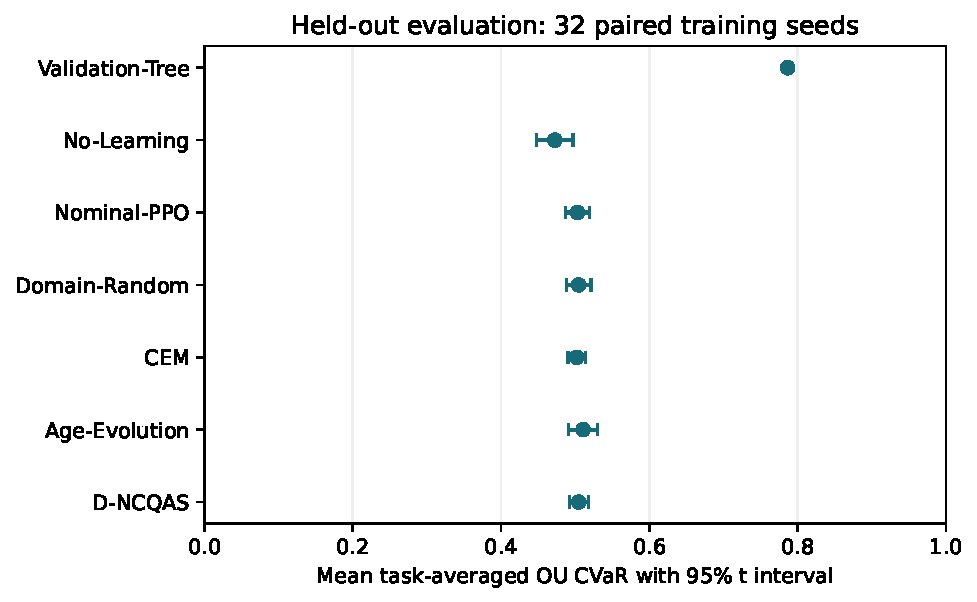
\includegraphics[width=.95\linewidth]{../outputs/analysis/figures/fig10_paper_aggregate.pdf}\caption{Main held-out task-averaged tail fidelity. Intervals summarize variability across 32 independent training seeds; tasks are fixed.}\end{figure}
\begin{figure}[htbp]\centering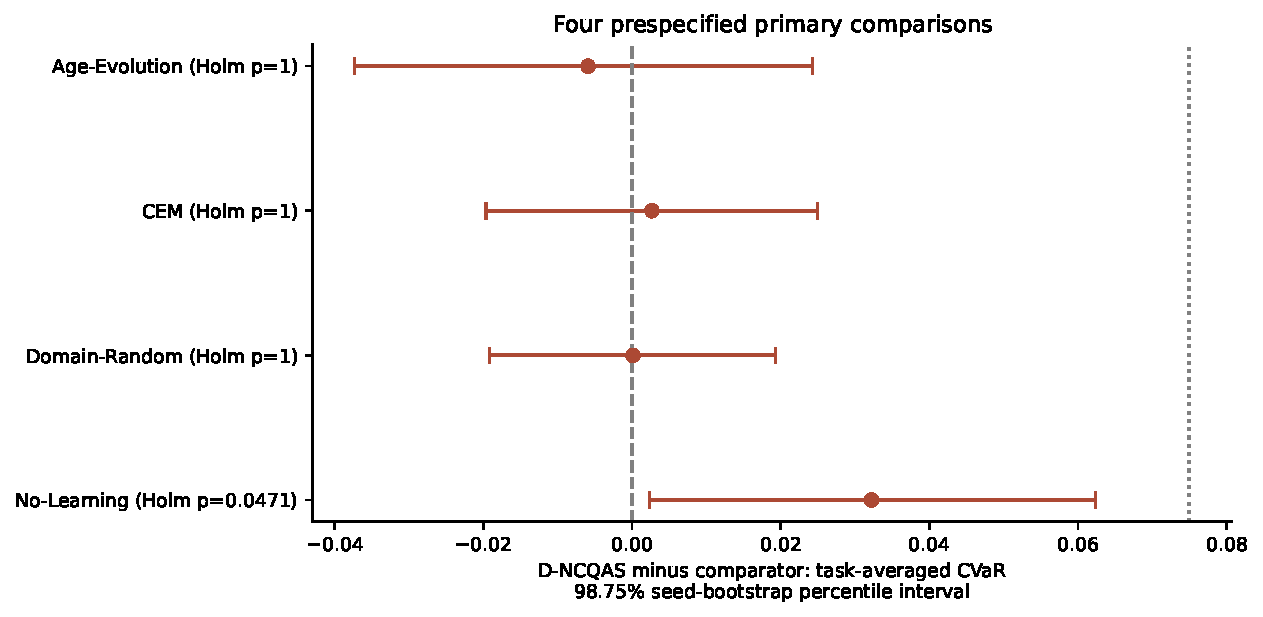
\includegraphics[width=.98\linewidth]{../outputs/analysis/figures/fig4_primary_effects.pdf}\caption{Four primary paired contrasts. Dotted vertical line denotes the effect size used for planning; the dashed line denotes zero. Intervals are approximate 98.75 percent seed-bootstrap intervals.}\end{figure}
\begin{figure}[htbp]\centering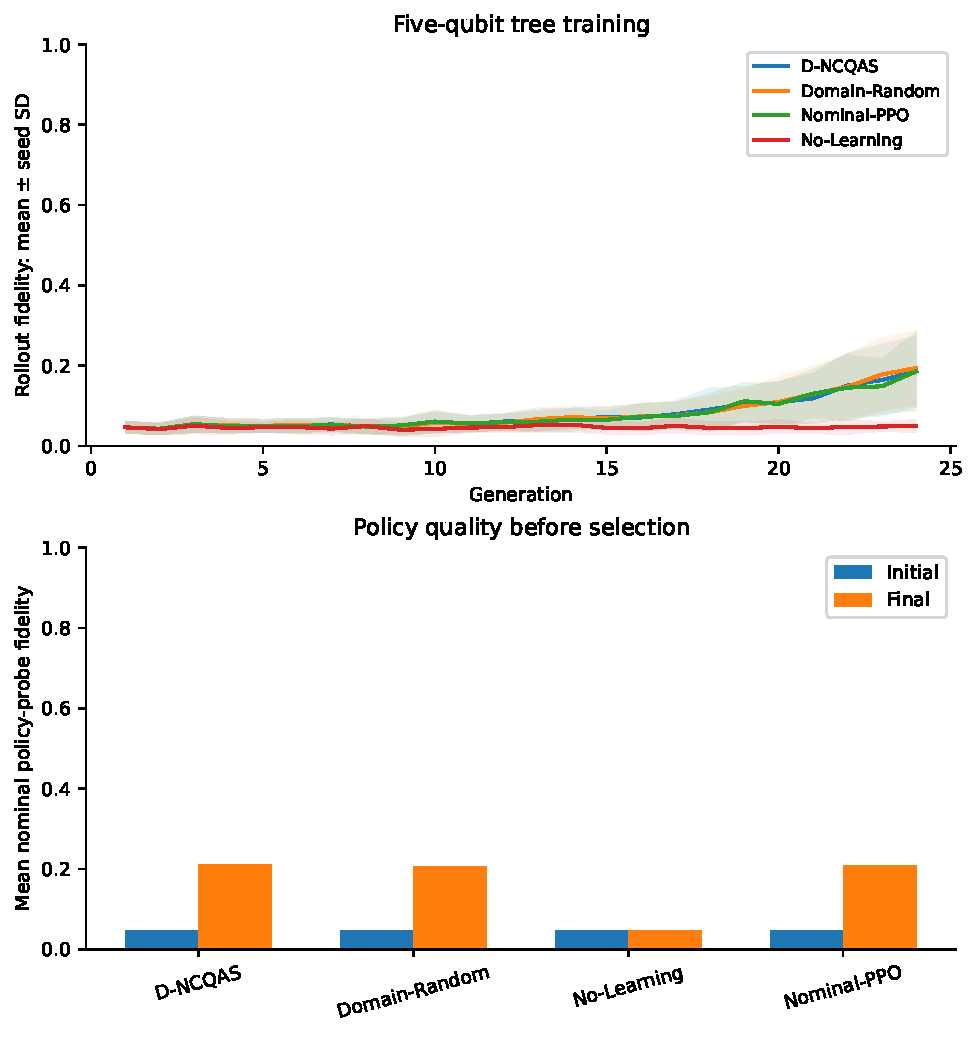
\includegraphics[width=.98\linewidth]{../outputs/analysis/figures/fig5_learning_and_probes.pdf}\caption{Five-qubit tree learning and independent policy probes. Training ribbons show seed standard deviations. Policy samples and validation-selected circuits are different estimands.}\end{figure}

\section{Molecular provenance and convergence study}
The molecular component remains a separate fixed-ansatz validation. PySCF \cite{pyscf} generates RHF/STO-3G integrals at H2 0.735 angstrom, HeH+ 0.775 angstrom with charge +1, and LiH 1.6 angstrom. CAS(2,2) retains one alpha and one beta electron in two active spatial orbitals; LiH freezes its core. The compact two-qubit CI basis indexes the occupied alpha and beta orbitals. Nuclear and core energies are included directly, without fitting a scalar shift to a target energy. Saved integrals support an independent fermionic reconstruction, and the matrix ground energies agree with active-space FCI. This is not a four-qubit Jordan-Wigner noise model, and LiH's reference is not full-molecule FCI.

One- and two-layer RY/CNOT circuits are fitted to clean or nominal-noise objectives for ten fresh seeds and five matched starts. Each setting compares COBYLA with 400 and 2000 function-evaluation caps and BFGS with a parameter-shift Jacobian and a 2000-iteration limit. The BFGS branch is designated as the final estimator before inspecting test energies. All starts, statuses, objective values and parameters are retained. An independent maximum-gradient threshold of 1e-6 Ha/radian defines stationarity; solver success is reported separately. The parameter-shift Jacobian is checked against central finite differences for all three matrices under nominal noise.

All 120 selected BFGS fits pass the stationarity criterion; 112 report solver success. The largest selected gradient norm is 2.61e-08 Ha/radian. Table 3 shows both termination and stationarity rates for every optimizer branch, so numerical precision warnings are not hidden. Stationarity does not prove a global minimum. Selected angles are frozen for one clean evaluation and 100 draws per noisy regime, yielding 36,120 observations. Physical energy and assignment-noisy measured energy are distinct; only the physical expectation is constrained by the Hamiltonian variational bound. Measurement basis rotations are ideal and shot noise is absent.
\begin{table}[htbp]\centering\small\caption{Selected-fit convergence diagnostics over 120 molecular fits. The independent stationarity threshold is $10^{-6}$ Ha/radian.}\begin{tabular}{lrrr}\toprule
Optimizer/cap & Solver success & Stationarity & Maximum gradient\\\midrule
BFGS/2000 & 93.3\% & 100.0\% & 2.61e-08\\
COBYLA/400 & 50.8\% & 50.8\% & 0.000303\\
COBYLA/2000 & 50.8\% & 50.8\% & 0.000146\\
\bottomrule\end{tabular}\end{table}
\begin{figure}[htbp]\centering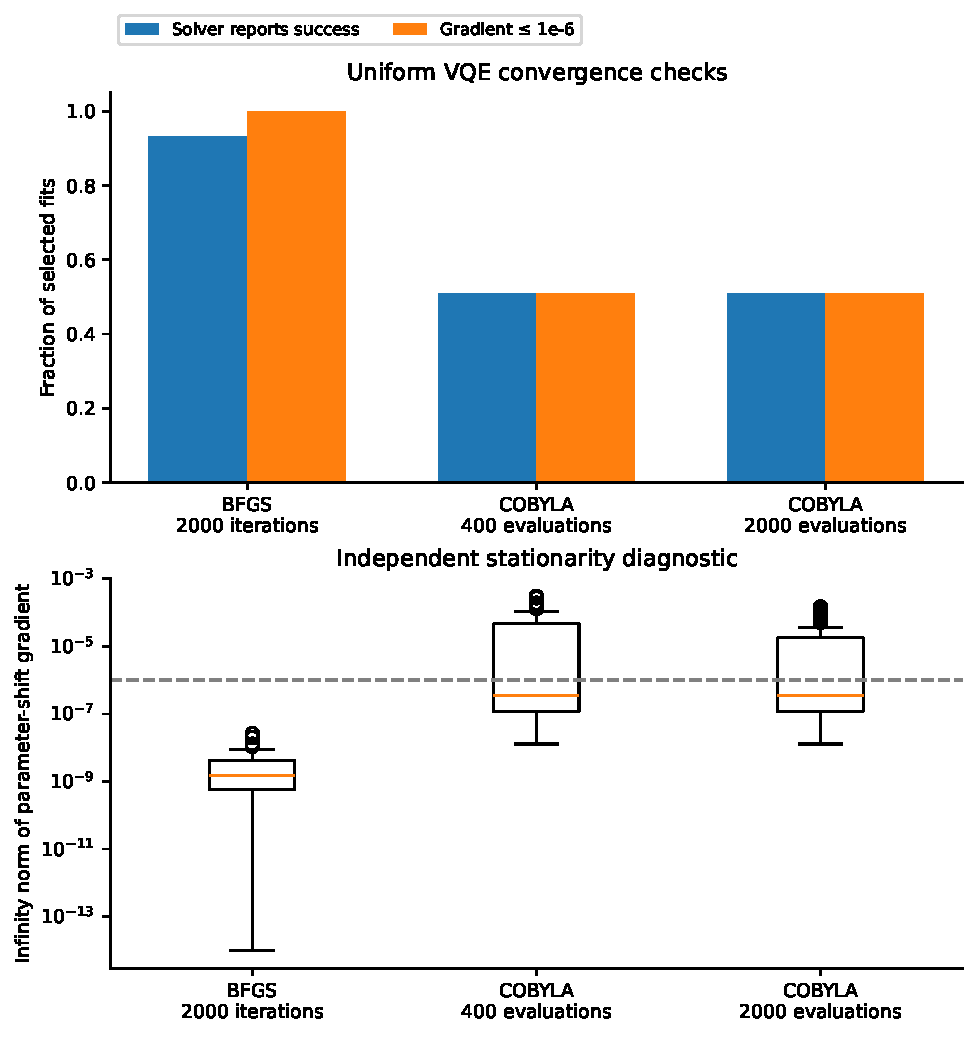
\includegraphics[width=.98\linewidth]{../outputs/analysis/figures/fig6_vqe_convergence.pdf}\caption{Molecular convergence across all 120 selected fits. Solver success and gradient stationarity are reported separately; increasing the COBYLA cap alone does not establish stationarity.}\end{figure}

\section{Limitations and interpretation}
The contribution is a reproducible controlled diagnosis, not a new state-of-the-art QAS algorithm. The graphs, rates and drift processes are synthetic, the main tasks contain only three or five qubits, and there are no QPU, real-calibration, shot-noise or mitigation experiments. The final inference is conditional on three fixed tasks and a development-selected configuration. A stronger benchmark would reproduce specialized QAS implementations such as those discussed above under compatible budgets and noise models. Our generic CEM/evolution controls supply useful independent references but do not establish that coverage.

The planning model targets a relatively large effect; smaller differences may remain uncertain. A 100-draw tail estimate contains twenty full lower-tail samples and is not a tail-sample convergence study. The shared validation bank is used for candidate selection and therefore contributes search effort. Limited observability, reward shaping, minimum circuit length and the action grammar can influence search behavior. We have not isolated all such mechanisms causally. The known difficulty of fidelity-only rewards \cite{trap} provides context, not proof that the same mechanism fully explains every run. No final outcome is used to redesign the primary hypothesis family. Molecular stationarity under exact simulation does not establish chemical accuracy under realistic device noise.

\section{Reproducibility, availability and conclusion}
The release contains 108 development jobs, 672 main search jobs, 64 secondary ablation jobs, and 120 molecular fits with all optimizer branches. Twenty numerical/regression tests check gradients, policy probabilities, frozen controls, stress budgets, graph legality, channels, pairing, molecular construction and parameter-shift derivatives. The verifier checks every configured job and raw summary, shared scenario identifiers, source/protocol hashes, selected full-bank replays and the molecular stationarity requirement. Exact dependency locks and executable analysis scripts accompany the data. Notebook cells are validated sequentially in-process; live Colab is not claimed tested.

Only the frozen-policy contrast favors D-NCQAS after Holm correction (difference +0.0322; adjusted p=0.0471); the other three primary contrasts are not significant. Optimizer diagnostics and independent controls make the limits of the search results assessable, while the convergence study replaces capped molecular estimates with explicitly checked stationary fits. The evidence supports the stated finite-study conclusions and provides a reusable basis for larger or hardware-specific work. It does not warrant a universal superiority claim. Code is distributed under MIT with retained attribution. This anonymized draft uses AI assistance for code revision, experiment orchestration and writing; submitting authors must verify the final claims and complete authorship, funding, conflict, repository and venue-specific declarations.

\appendix
\section{Reproduction settings}
The architect uses Adam learning rate 0.001, beta1=0.9, beta2=0.999, epsilon=1e-8, PPO clip 0.2, entropy coefficient 0.02, discount 0.99, GAE lambda 0.92 and three full-batch update epochs per generation. Per-parameter gradients are clipped to [-1,1] after batch averaging. The critic uses a scaled Huber derivative. The saboteur trains on the first stress sample in eight episodes per generation. Every model starts from seed-specific independent random streams. Candidate selection uses 20 validation OU draws and tail mass 0.20. Main testing uses 100 draws per regime. Exact generation inputs, molecular orbitals, Hamiltonian matrices, random states and parameters are in the archive.
Nominal one-qubit, edge and assignment rates are 0.001 times linspace(0.8,1.4,n), 0.010 times linspace(0.75,1.75,|E|), and 0.020 times linspace(0.8,1.5,n). Training OU parameters are kappa=0.35, sigma=0.28, aging shift=0.22, burst probability per unit time=0.06 and dt=0.25. Held-out OU uses 0.30, 0.42, 0.35, 0.12 and 0.30 respectively, with a spatial permutation on every fourth draw. The last of six calibration snapshots is used. Static and OU testing amplify one-qubit and assignment rates by independent uniform factors in [1,2] and each edge rate by a factor in [1,4]. These held-out stress draws are not projected to the training adversary budget; they test the explicitly specified wider distribution. Nominal testing uses independent category-level factors in [0.95,1.05]. Exact clipping, cross-component correlations, burst distributions and channel conventions are specified by the released simulator and scenario generator. The penalty uses logical depth obtained by advancing the layer counters of each touched qubit. Physical noise execution remains serial, so this depth is a structural penalty rather than the simulated elapsed duration. Reported train times include parallel-worker contention. The entropy calculation uses a numerical logarithm floor of 1e-8.

\begin{thebibliography}{99}
\bibitem{qas} E.-J. Kuo, Y.-L. L. Fang, and S. Y.-C. Chen, Quantum Architecture Search via Deep Reinforcement Learning, arXiv:2104.07715 (2021). \url{https://arxiv.org/abs/2104.07715}.
\bibitem{coev} J. Urbaneja et al., A Coevolutionary Framework for Noise-Resistant Quantum Architecture Search, ISC High Performance (2026). DOI: 10.23919/ISC.2026.11520504. \url{https://doi.org/10.23919/ISC.2026.11520504}.
\bibitem{bench} A. Ikhtiarudin, A. Das, P. Thakkar, and A. Kundu, BenchRL-QAS: Benchmarking reinforcement learning algorithms for quantum architecture search, AAAI Symposium Series (2025), arXiv:2507.12189. \url{https://arxiv.org/abs/2507.12189}.
\bibitem{trap} X.-Y. Bi, Y.-M. Yu, Y.-H. Chen, and Z.-R. Zhong, General-purpose quantum architecture search based on deep reinforcement learning, Physical Review A 112, 052409 (2025). \url{https://doi.org/10.1103/7rc4-p446}.
\bibitem{ppo} J. Schulman et al., Proximal Policy Optimization Algorithms, arXiv:1707.06347 (2017). \url{https://arxiv.org/abs/1707.06347}.
\bibitem{adam} D. P. Kingma and J. Ba, Adam: A Method for Stochastic Optimization, arXiv:1412.6980 (2014). \url{https://arxiv.org/abs/1412.6980}.
\bibitem{cem} P.-T. de Boer, D. P. Kroese, S. Mannor, and R. Y. Rubinstein, A Tutorial on the Cross-Entropy Method, Annals of Operations Research 134, 19-67 (2005). \url{https://doi.org/10.1007/s10479-005-5724-z}.
\bibitem{evolution} E. Real, A. Aggarwal, Y. Huang, and Q. V. Le, Regularized Evolution for Image Classifier Architecture Search, AAAI (2019), arXiv:1802.01548. \url{https://arxiv.org/abs/1802.01548}.
\bibitem{cvar} P. K. Barkoutsos et al., Improving Variational Quantum Optimization using CVaR, Quantum 4, 256 (2020). \url{https://doi.org/10.22331/q-2020-04-20-256}.
\bibitem{pyscf} PySCF project, FCI and molecular-structure documentation, accessed 20 October 2026. \url{https://pyscf.org/pyscf_api_docs/pyscf.fci.html}.
\end{thebibliography}
\end{document}
